\begin{frame}{Next steps}
  We consider the current state of the program mostly production-ready with few
  exceptions

  \vspace{\baselineskip}

  \begin{itemize}
  \item[--] \textbf{Get subgroup members to start editing system components}
  \item[--] Drag calculations are long and can be offloaded to a dedicated
    module
  \item[--] Materials module rewrite with Rishabh's new code
  \item[--] Lots of small details need fixing in individual modules
  \item[--] Better naming?
  \end{itemize}
\end{frame}

\begin{frame}{Calculations people}
  \begin{figure}
  \captionsetup{labelformat=empty}
  \begin{minipage}{0.3\linewidth}
    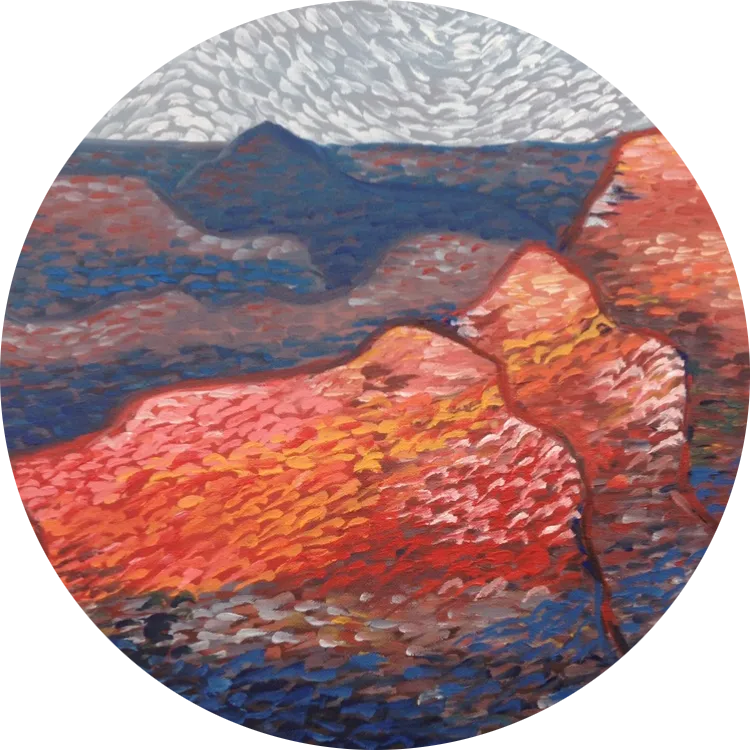
\includegraphics[width=\textwidth]{figures/andrii-avi.png}
    \caption{Andrii}
  \end{minipage}
  \hfill
  \begin{minipage}{0.3\linewidth}
    
\includegraphics[width=\textwidth]{figures/noa-avi.png}
    \caption{Noa}
  \end{minipage}
  \hfill
  \begin{minipage}{0.3\linewidth}
    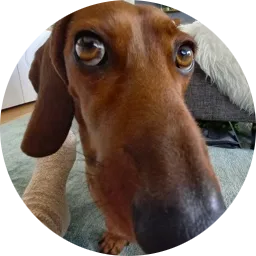
\includegraphics[width=\textwidth]{figures/sophia-avi.png}
    \caption{Sophia}
  \end{minipage}
  \end{figure}
\end{frame}


\begin{frame}{Next steps}
  \justifying

  Once the current calculations program is fleshed out, we will proceed with
  merging the solver with BEARS' flight sim program \lstinline{rocketpal} on a
  new branch, while master with the current structure remains for support

  \center{
    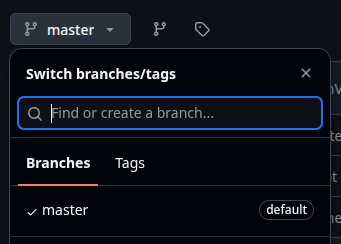
\includegraphics[width=0.5\columnwidth]{figures/branches.png}
  }
\end{frame}

\begin{frame}{Integration plan}
  \centering
  \resizebox{\textwidth}{!}{
    \begin{tikzpicture}[
      %transform canvas = {scale=0.6},
      node distance    = 8mm,
      s/.style         = {font=\ttfamily}
    ]
    % Inputs
    \node (inp) at (-6, 0) [s] {Inputs};

    \node (inp1) [
      s, draw, below=of inp.south,  anchor=south, minimum width=4cm
    ] {Rocket Parameters};

    \node (inp2) [
      s, draw, below=of inp1.south,  anchor=south, minimum width=4cm
    ] {Chemistry};

    \node (inp3) [
      s, draw, below=of inp2.south,  anchor=south, minimum width=4cm
    ] {Flight Parameters};

    \node[draw, fit={(inp) (inp1) (inp2) (inp3)}] (inpt) {};

    % Solver
    \node (solv) at (0, 0) [s] {OpenMDAO Solver};

    \node (solv1) [
      s, draw, below=of solv.south,  anchor=south, minimum width=3cm
    ] {Sizing};

    \node (solv2) [
      s, draw, below=of solv1.south, anchor=south, minimum width=3cm
    ] {Optimization};

    \node[draw, fit={(solv) (solv1) (solv2)}] (solvt) {};

    % Simulator
    \node (sim) at (0, -4) [s] {RocketPy Simulator};

    \node (sim1) [
      s, draw, below=of sim.south,  anchor=south, minimum width=5cm
    ] {Flight Sim};

    \node (sim2) [
      s, draw, below=of sim1.south, anchor=south, minimum width=5cm
    ] {Monte Carlo Dispersion};

    \node (sim3) [
      s, draw, below=of sim2.south, anchor=south, minimum width=5cm
    ] {Stability};

    \node[draw, fit={(sim) (sim1) (sim2) (sim3)}] (simt) {};

    % Outputs
    \node (out) at (7, -4) [s] {Outputs};

    \node (out1) [
      s, draw, below=of out.south,  anchor=south, minimum width=6cm
    ] {Optimized Rocket Parameters};

    \node (out2) [
      s, draw, below=of out1.south, anchor=south, minimum width=6cm
    ] {Flight Sim Outputs (TBD)};

    \node[draw, fit={(out) (out1) (out2)}] (outt) {};

    % Connections
    \draw[->] (inpt) -- (inpt.east -| solvt.west);
    \draw[->] (inpt.south) to [bend right] (simt.west);

    \draw[->] (solvt) -- (simt) node[
      style={font=\ttfamily\small}, midway, right
    ] {Optimized rocket parameters};

    \draw[->] (simt.east |- outt.west) -- (outt.west);
    \end{tikzpicture}
  }
\end{frame}
